\documentclass[
    DIV12,
    cleardouble=plain,
    headings=normal,
    pdftex,
    headexclude,footexclude,
    final
]{scrreprt}

\usepackage{spreadtab}
\usepackage{xspace}
\usepackage[ngerman]{babel}
\usepackage[utf8]{inputenc}
%\usepackage[T1]{fontenc}
\usepackage[pdftex]{graphicx}
\usepackage[bookmarks]{hyperref}
\usepackage{scrpage2}
\usepackage{longtable}
\usepackage{caption}
\usepackage{pgfplots}
\usepackage{float}
\usepackage{xcolor}
\usepackage{colortbl}
\usepackage{tabularx}
\usepackage{multirow} % tabelle
\usepackage{listings} % code aus datei einbinden
\usepackage{scrhack}
% \usepackage{minted} % package for swift

% Swift language definition
\lstdefinelanguage{Swift}{
  keywords={associatedtype, class, deinit, enum, extension, func, import, init, inout, internal, let, operator, private, protocol, public, static, struct, subscript, typealias, var, break, case, continue, default, defer, do, else, fallthrough, for, guard, if, in, repeat, return, switch, where, while, as, catch, dynamicType, false, is, nil, rethrows, super, self, Self, throw, throws, true, try, associativity, convenience, dynamic, didSet, final, get, infix, indirect, lazy, left, mutating, none, nonmutating, optional, override, postfix, precedence, prefix, Protocol, required, right, set, Type, unowned, weak, willSet},
  ndkeywords={class, export, boolean, throw, implements, import, this},
  sensitive=false,
  comment=[l]{//},
  morecomment=[s]{/*}{*/},
  morestring=[b]',
  morestring=[b]"
}

% word wrap with a red arrow
\lstset{
  basicstyle=\ttfamily,
  columns=fullflexible,
  frame=single,
  breaklines=true,
  postbreak=\mbox{\textcolor{red}{$\hookrightarrow$}\space},
}

\graphicspath{{./}{./images/}}

% #################################################################

\hyphenation{Cha-otn-gsch-werl}
\setlength\headheight{1.75cm}

\ihead{\small{Hochschule Hof}}
\chead{}
\ohead{
\includegraphics[height=0.05\textheight]{fh_logo}}
\pagestyle{scrheadings}


\setcounter{secnumdepth}{5}
\setcounter{tocdepth}{5}
\renewcommand{\arraystretch}{1}

\parskip0.5\baselineskip plus 0.125\baselineskip minus 0.25\baselineskip
\parindent0em

%\automark[section]{chapter}

\titlehead{\begin{center}
\includegraphics[width=5cm]{fh_logo}\end{center}}
 \title{
  Stundenplan--App v4 für iOS \\[1em]
  Dokumentation, Spezifikation, Konstruktion
}

\author{}
\date{xx.xx.2018} %##Abgabedatum einfügen

% #################################################################


\begin{document}
\maketitle
\pagenumbering{roman}
\tableofcontents

%\listoftables

\newpage
\pagenumbering{arabic}

%hier die einzelnen Punkte einfügen
\chapter{Projektablauf}
Johannes Franz \& Christian Pfeiffer

\section{Ausgangssituation}
%%todo: Beschreiben, dass die iOS App schon von unseren Vorgängern entwickelt worden ist und welche Funktionen diese (V1,V2,V3) hattte

Im Wintersemester 2016/2017 begann die Entwicklung der iOS Stundenplanapp mit Studierenden des Studiengangs Mobile Computing im 5. Semester im Rahmen des Moduls "Fortgeschrittene Themen der Swift 3 Programmierung". Am Ende dieses Semesters wurde die Version V1 im AppStore veröffentlicht. Im Sommersemester 2017 wurde die App weiterentwickelt und schlussendlich die Version 2.0 veröffentlicht, welche eine Background Fetch Funktionalität einführte, lokale Notifications bei Vorlesungsverlegungen und Verbesserungen bei der Erkennung von einzelnen Vorlesungsterminen integrierte..

Im Wintersemester 2017/2018 übernahmen unser Studienjahrgang (Studierende des 5. Semesters) im Rahmen des Moduls "Fortgeschrittene Themen der Swift 3 Programmierung" die Pflege und Weiterentwicklung der iOS Stundenplanapp.


\newpage
\section{Überlegungen zu Projektbeginn}

\subsection{GitHub / Branches}
GitHub ist eine Plattform zur effektiven Versionsverwaltung von Softwareprojekten. Branches stellen gewisse Softwareversionen dar. Das Verwenden mehrerer Branches ermöglicht es größeren Softwareteams gleichzeitig an verschiedenen Softwarefeatures zu arbeiten.
Für die iOS Stundenplanapp wurde ein passendes Branch-Konzept vom Projektmanagment Team ausgearbeitet.

Der Großteil der Kommunikation lief über Issues und den Project Tab von GitHub ab.

\subsubsection{Ausgangslage}

Zu Projektbeginn waren folgende Branches vorhanden:
\begin{itemize}
\item master
\item development (obsolete)
\item v2 (depricated)
\item v3 (aktuell auf Deployment Target 10.0 entspricht iOS Version 10)
\end{itemize}


Von den vorherigen Projektteams wurde in GitHub ein Wiki angelegt.
Link zum Wiki:\\
\url{https://github.com/HochschuleHofStundenplanapp/iOS-App/wiki}

Darin wurden in kurzer Form einige Auszüge aus den jeweiligen PDF Dokumenten zusammengetragen.




GitHub Branch Übersicht:\\
 \url{https://github.com/HochschuleHofStundenplanapp/iOS-App/branches}

\subsubsection{Verbesserungen}
Es wurde beschlossen, die vorherige Struktur beizubehalten. Dabei wurden Branches jeweils mit der Versionsnummer beschriftet.

Der "master" Branch wird immer mit der aktuellsten Version gefüllt.

Neue Branches sind eingeführt worden:
\begin{itemize}
\item v3.1: (Bugfixes, kleinere neue "Features". Der Branch bleibt auf Swift 3.1  / iOS 10.0)
\item v3.2: Weitere Bugfixes. Der Branch bleibt auf Swift 3.1  / iOS 10.0 %%##todo
\item v4: in Rahmen der Studienarbeit entwickelte Erweiterungen der App (Swift 4 / iOS 11)
\item v4-widget: Subbranch der v4 zur Anpassung der App an ein Framework, welches
Vorraussetzung für die Implementierung eines Widget war.
\end{itemize}
\newpage
Veränderungen an bestehenden Branches:
\begin{itemize}
\item master: Der master Branch beeinhaltet immer die aktuell ausgelieferte Version aus dem Appstore.
\item development: Der development Branch wurde als obsolet gekennzeichnet und deshalb entfernt.
\end{itemize}


Es wurde von der Projektgruppe entschieden beim iOS 10 Deployment Target zu bleiben, da zu Beginn des Semester iOS 11 erst veröffentlicht wurde und die Verteilung erst ein paar Monate dauerte. Zudem wurde für einige ältere Geräte, wie dem iPhone 5, iPhone 5C, and iPad 4, der Support eingestellt, weshalb einige Studierende keine App Updates mehr erhalten würden.

Letztendlich wurde entschieden das Projekt auf Swift 4 zu aktualisieren. Dies brachte u.a. Effizienzverbesserungen bei der String Manipulation. Diese wird beispielsweise in der Artificial Intelligence Klasse verwendet.

Zu Projektbeginn entstand die Idee, Branches nach Features zu benennen. Dabei war Design, Siri, Kalendersynchronisation, etc. angedacht. In der Projektphase hat sich zwischenzeitlich bewährt, Branches weiterhin nach Versionsnummern zu benennen und bei großen Änderungen der Versionsnummer ein Thema anzuhängen.


\section{Ziele für Version 4}
Folgende Aufgaben wurden als Ziel für die Version 4 festgelegt:
% Jede Funktion kurz Beschreiben, was es tut... Warum wir es brauchen Add Siri, weil ist ja dokumentiert - cpfeiffer
\begin{itemize}
\item Migration des Projektes auf Swift 4
\item Onboarding
\item Hausaufgaben Manager
\item Push Notifications
\item Widget
\item iOS 11 Design
\item Testkonzept für die App
\item Auslagerung des Appmodels in ein Framework
\item Parsen von vorlesungsfreien Tagen von der HS Webseite
\end{itemize}

\newpage
\section{Teams}

Team 1: (Pfeiffer, Scheler)
\begin{itemize}
\item Design
\item Buxfixes
\item Swift 4 Konvertierung
\item Universal App Color Persistenz
\item Design des Onboarding
\end{itemize}


Team 2: (Franz, Krug):
\begin{itemize}
\item Siri
\item Implementierung von Push Notifications
\item Erweiterung der Schnittstelle
\end{itemize}


Team 3: (Hagmann, Knoblauch, Niepel):
\begin{itemize}
\item Verschiedene Fehlerbehebungen
\item Hausaufgaben Manager
\item Onboarding 
\item Universal App Color
\item Kalenderschnittstelle überarbeitet
\end{itemize}


Team 4: (Kusserow, Sonntag, Dümmlein):
\begin{itemize}
\item Stundenplan Verbesserungen
\item Erstellen eines Widgets
\item Auslagerung des Appmodels in ein Framework
\item Parseen von vorlesungsfreien Tagen von der HS Webseite
\end{itemize}


Team 5: (Pöhlmann):
\begin{itemize}
\item Testkonzept ausarbeiten
\item Testen nach Protokoll
\end{itemize}

\newpage
\section{Kommunikation}
Zur Verständigung untereinander und Festlegung der einzelnen Aufgaben wurden verschiedene Kommunikationsarten und Plattformen verwendet.
\begin{itemize}
\item Chat Gruppe mit allen Beteiligten
\item Kommunikation während der Zeit in der Hochschule
\item GitHub (Issues, Project Tab)
\item Scrum ähnliche Vorstellung neu eingebauter Funktionen zu Beginn jeder Vorlesung
\end{itemize}


\section{Projektfortschritt dokumentiert}
Unter Zuhilfenahme des Projektfeature in GitHub konnte immer der Überblick über Subtasks der einzelnen Teams behalten werden und so der Fortschritt der Gruppen dokumentiert werden.

Projekt Tab in GitHub\\
\url{https://github.com/HochschuleHofStundenplanapp/iOS-App/projects}






\section{Fazit und Ausblick}
Zu Beginn des Semesters wurden die Nutzer  mit Service Updates und Fehlerbehebungen versorgt. Hierfür entstanden die Versionen V3.1 und V3.2, welche die Stabilität der Stundenplanapp verbesserten und akute Probleme wie das Fehlen des roten Beschreibungstextes bei Stundenplanänderungen behob.

Bis zum Ende des Semesters waren wir in der Lage alle zielgesetzten Funktionalitäten in die V4 zu implementieren. Nur noch kleine Änderungen und die Übergabe der Server Komponente an den IT-Service zum Updaten der Produktiv Server Umgebung verzögerten die Veröffentlichung in den Appstore.
Wie auch bei der vorherigen Version werden zu Beginn des Sommersemester 2018 weitere Qualitätsverbesserungen und Fehlerbehebungen vorgenommen  werden müssen, damit die neue Version bei den Endnutzern als abgerundetes Produkt ankommt.
\chapter{Design}
Angelina Scheler \& Christian Pfeiffer

\section{Einleitung}
Eine weitere Aufgabe, die unsere Gruppe übernommen hat, war das Onboarding für die Stundenplan App. Im Onboarding kann der Nutzer gleich zum Start der App seine Einstellungen zu Fakultät, Studiengang, Semester, Vorlesung und Kalendersynchronisation vornehmen. Das Onboarding wird gestartet, wenn noch keine Angaben zu den genannten Einstellungen gemacht wurden.

\begin{itemize}
\item Neues Design
\item besseres Design
\item iOS Design
\end{itemize}

\begin{enumerate}
\item Fakultät (die die Farbe der App bestimmt)
\end{enumerate}


\section{Stundenplan}
Unsere Design Sachen sind sehr schön!
\subsection{Screen1}

\begin{figure}[ht]
	\centering
  \frame{ 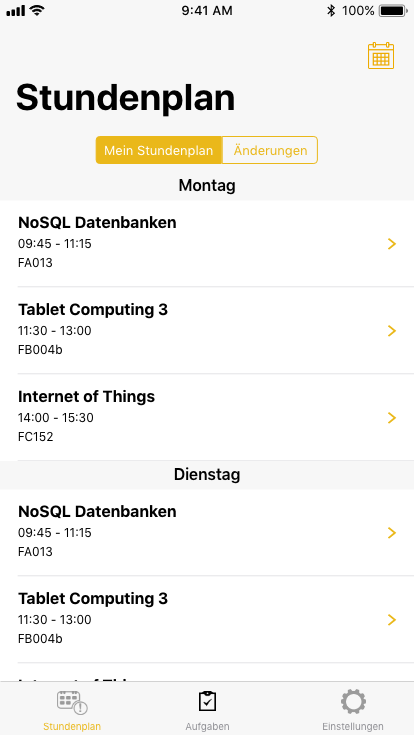
\includegraphics[width=0.3\textwidth]{Mein_Stundenplan} }
	\caption{Mein schönstes Mockup}
	\label{fig1}
\end{figure}

\section{Onboarding}
\section{Einstellungen}
\section{Widget}

\section{demo}
Eine weitere Aufgabe, die unsere Gruppe übernommen hat, war das Onboarding für die Stundenplan App. Im Onboarding kann der Nutzer gleich zum Start der App seine Einstellungen zu Fakultät, Studiengang, Semester, Vorlesung und Kalendersynchronisation vornehmen. Das Onboarding wird gestartet, wenn noch keine Angaben zu den genannten Einstellungen gemacht wurden.

\begin{itemize}
\item Neues Design
\item besseres Design
\item iOS Design
\end{itemize}

\begin{enumerate}
\item Fakultät (die die Farbe der App bestimmt)
\end{enumerate}

\begin{figure}[ht]
	\centering
  \frame{ 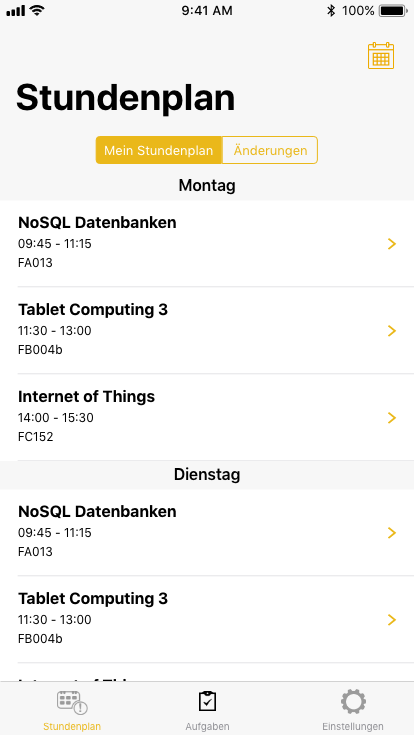
\includegraphics[width=0.4\textwidth]{Mein_Stundenplan} }
	\caption{Mein schönstes Mockup}
	\label{fig2}
\end{figure}


\chapter{Siri Probleme}


\section{Überschrift A}
Hier könnte etwas über Siri stehen\\


\newpage
\section{Überschrift B}
Hier könnte noch mehr über Siri stehen\\


\section{Überschrift B}
Hier könnte noch viel mehr über Siri stehen\\
\chapter{Push Notifications}
Johannes Franz \& Normen Krug

\section{Einleitung}
Push Notifications sind ein fester Bestandteil moderner Apps. Deswegen soll die Stundenplan App um solche erweitert werden. Ziel soll es sein den Benutzer über Stundenplanänderungen aktiv zu informieren, um speziell auf kurzfristige Änderungen reagieren zu können. Ein Server überprüft dabei eine Stundenplan Datenbank auf Änderungen und sendet eine Push Notification an alle iOS Geräte, die sich für die jeweilige Vorlesung registriert haben. Ein Apache Webserver stellt dabei mit einer MySQL Datenbank und entsprechenden Chronjobs das Backend bereit.

GitHub repository: \url{https://github.com/HochschuleHofStundenplanapp/iOS-App/}


\section{Projektablauf}
Um den Projektfortschritt nachvollziehen zu können, wurde dieser tabellarisch in Verbindung mit dem aktuellen Datum aufgelistet.


\noindent%
\begin{tabularx}{\textwidth}{|p{.25\textwidth}|X| }
\hline
\textbf{Datum} & \textbf{Erreichter Meilenstein}  \\ \hline 

Vorlesungsbeginn & Themenfindung \\ \hline

Siri & Einarbeitung in Siri. Erkennen erster Hürden. \\ \hline

Neue Themenfindung & Verwerfen von der Siri Projektidee und neue Themenfindung. \\ \hline

Festlegung & Thema Push Notifications festgelegt und Beginn der Einarbeitung. \\ \hline

28.10.2017 & Push Notifications lassen sich per PHP Script an einen fest eingestellten Token schicken \\ \hline

30.10.2017 & Eine Test iOS App kann per php Script mittels MAMP lokal eine Push Notification senden. \newline
Datenbank lokal in PhpMyAdmin angelegt. \newline
PHP Script schreibt bei Aufruf in die angelegte SQL Datenbank. \newline
Einarbeitung und Konvertierung der Dokumentation in Latex.
 \\ \hline
 31.10.2017 & Die Test iOS App wurde so erweitert, dass ein JSON File per POST Nachricht übermittelt werden kann.\newline
Das PHP Script parst nun das ankommende JSON File und fügt per insert die geparsten Daten in die Datenbank ein.\newline 
Einarbeitung in bestehende Schnittstelle und Überlegungen wie das bestehende Backend erweitert werden muss. 
 \\ \hline
 

Zwischenzeit & PHP Scripte der bestehenden (Android) Schnittstelle angepasst und getestet. \newline
\\ \hline 
 
 
24.11.2017 & Testserver wurde bereitgestellt. \newline
\\ \hline 
 
 
2018 & Push Notifications mit HTTP2 implementiert.
\newline
\\ \hline  

\end{tabularx}

\newpage


\section{Vorbereitung einer Testumgebung}

\subsection{MAMP als Virtuelle Umgebung}

\subsubsection{MAMP}
Die Testumgebung MAMP (Akronym steht für: Mac, Apache, MySQL, PHP) virtualisiert die genannten Komponenten, um lokale Tests zu ermöglichen.


\subsubsection{MySQL Datenbank}

Die Tabelle \textit{fcm\_nutzer} enthält eine Zuordnung von abonnierten Vorlesungsverlegungen mit dem jeweiligen Token des Gerätes. Dabei ist zusätzlich vermerkt welches Betriebssystem verwendet wird. Die \textit{0} in der Spalte \textit{os} steht dabei für Android während \textit{1} iOS repräsentierts. \\
Da die ausgewählte Sprache des Nutzers nicht bekannt ist, wird für die \textit{language} Spalte an dieser Stelle auch null akzeptiert. Um bei einer späteren Version der App zwischen Nutzern die noch keine Sprache ausgewählt haben und allen anderen differenzieren zu können, wird hier trotz der aktuell nur in deutsch vorhandenen App der Wert nicht standardmäßig auf deutsch gesetzt.
\lstinputlisting[language=SQL]{content/pushNotifications_create.sql}
Da eine bestehende Infrastruktur die Grundlage dieses Projektes darstellt, musste diese Tabelle lediglich um \textit{os} und \textit{language} erweitert werden.\\
Auf Änderungen an anderen Tabellen konnte komplett verzichtet werden.




\section{Umsetzung}
Apple bietet für die Umsetzung von Push Nachrichten den Apple Push Notification service (APNs) an. Dabei handelt es sich um einen bei Apple gehosteten Dienst, der Push Notifications per API ermöglicht.


\subsection{Server Installation}
Zur Installation der Software sind Admin Rechte notwendig. Der \textit{wget} Befehl läd dabei eine zum aktuellen Zeitpunkt sehr neue \textit{curl} Version herunter. Diese hat die Besonderheit HTTP2 zu unterstützen, welches für die Push Notification Schnittstelle von Apple vorausgesetzt ist.
\lstinputlisting[language=bash]{content/pushNotifications_server_install.bsh}


\subsection{Zertifikate}
Um mit einer gesicherten Verbindung auf die Apple Push Notification Schnittstelle zuzugreifen, werden zwei Zertifikate benötigt. Dabei handelt es sich um ein öffentliches und privates Zertifikat. Diese Zertifikate müssen vor der Verwendung in das Zielformat \textit{.pem} umgewandelt werden, bevor sie benutzbar sind.

Um die Zertifikate zu anzulegen und zu verwalten, stellt Apple eine Übersicht dem bei Apple angemeldeten Entwickler bereit. Bei dem verwendeten Zertifikat wird zwischen \textit{Development} und \textit{Production} unterschieden.\\
\url{https://developer.apple.com/account/ios/certificate/}

\\
Die MacOS App ``Easy APNs Provider`` ermöglichte ersten Gehversuche, um Push Nachrichten an ausgewählte Token zu senden.\\
Quelle: \url{https://github.com/immobiliare/ApnsPHP}



\subsection{Code zum Registrieren am Server}
Um sich am Server für eine Vorlesung zu registrieren waren Veränderungen im Code notwendig.
\lstinputlisting[language=Swift]{content/pushNotifications_Swift_Example.swift}


\section{Aufgetretene Probleme}
Als Herausforderung zu sehende Punkte haben häufig sehr viel Zeit in Anspruch genommen oder den Projektfortschritt entschleunigt.


\begin{itemize}
\item Verzögerte Bereitstellung des Servers führte zu komplexen Reimplementierungen in schwer zu synchronisierenden getrennten VMs
\item Beschränkte Rechte auf dem Testserver die nach und nach erweitert werden mussten
\item Verschiedene Zertifikatarten sind sehr verwirrend
\item Bundle Identifier und App Capabilities mussten nach jedem Git Pull wieder angepasst werden
\item Komplexes Testen (Lokale Server, Erreichbarkeit im Labornetzwerk / Wi-Fi, unterschiedliche Datei- und Serverstände) 
\item Zu Beginn kein Zugriff auf die Git Schnittstellen Projekt
\item Ablaufende Zertifikate
\item Serverseitig unterschiedliche Übertragungsverfahren zwischen Android und iOS
\item Erschwertes Debugging der PHP Scripte
\item HTTP2 wurde von Apache2 und Curl nicht offiziell unterstützt
\item Struktur der Datenbank und der PHP Scripte war durch die Android App vorgegeben
\item Veraltete APNs Variante war stark verbreitet, brachte allerdings viele Probleme mit sich und musste als Ansatz letztendlich verworfen werden
\end{itemize}


\section{lessons learned}
Unser Team hat feststellen müssen, dass zu einem umfassenden iOS Projekt mehr als nur der Interface Builder und die Sprache Swift gehört. So sind Punkte zu nennen die positiv aus dem Projekt mitgenommen wurden.
\begin{itemize}
\item Linuxkenntnisse
\item PHP und Debugging auf dem Server
\item Beachten von Abhängigkeiten wie der Abwärtskompatibilität der Software zu früheren und bestehenden Android Versionen
\end{itemize}

\section{Weitere Arbeiten}
In diesem Projektabschnitt konnten alle gesteckten Ziele erreicht werden. Da solch ein relativ junges Projekt noch viele Möglichkeiten beinhaltet Funktionen zu verbessern und neue Funktionen einzuführen werden hier mögliche Punkte zur Anregung aufgelistet.

\begin{itemize}
\item Auswertungen die aktuell bei der Android und iOS App mehrfach auf dem Client Gerät stattfinden, können auf dem Server zentral bearbeitet werden. Dies verringert die Komplexität bei beiden Anwendungen und erleichtert die Wartung des Codes an zentraler Stelle.
\item Erweiterung der Push Notification Information um eine Priorität, Ablaufdatum,...
\item Aufkommende Issues und Ideen aus dem öffentlichen Git Projekt der iOS App und Schnittstelle
\item Erweiterung der App und Schnittstelle um andere Sprachen wie z.B. Englisch was in der Android App bereits angeboten wird

\end{itemize}


\chapter{Testen der Anwendung}
\section{Test des Widgets}
Philipp Dümlein \& Maximilian Sonntag \& Bastian Kusserow

\section{Testfälle}
Das Widget wurde über einen längeren Zeitraum getestet. Dabei wurden folgende Testfälle erarbeitet und überprüft:

\begin{itemize}
\item Aktuell keine Vorlesung - beide Vorlesungen in der nächsten Woche
\item Aktuell keine Vorlesung - nächste Vorlesung am darauffolgenden Tag
\item Aktuell keine Vorlesung - nächste Vorlesung in der nächsten Woche
\item Aktuell keine Vorlesung - nächste Vorlesung übermorgen
\item Aktuell eine Vorlesung - nächste Vorlesung nächste Woche
\item Aktuell eine Vorlesung - nächste Vorlesung am darauffolgenden Tag
\item Aktuell eine Vorlesung - nächste Vorlesung danach
\item Aktuell eine Vorlesung - nächste Vorlesung übermorgen
\end{itemize}


%usw. ...

\end{document}
